\section{Medical background}
The brain scans in the BraTS\cite{menze2015multimodal} 2018 dataset were made with MRI scanners\cite{mriscanner}.
The brain consists mostly of water. Water molecules contain two hydrogen molecules, each of which has one proton. A proton spins in a specific direction. When a strong magnet is applied to a proton, the proton starts to spin in the same direction as the magnet. 

A MRI scanner can generate a very precise and targeted magnetic field. When the magnet is deactivated, the protons go back into their resting position. Depending on the material a proton is part of (gray matter, necrotic tissue etc.), the resting position of the proton is different and a different amount of energy is released when the proton returns to its resting position. This energy is measured by the MRI scanner and visualized as a scan. MRI scans go trough the brain in layers and generate a 2D image of every layer called a slice. The output of an MRI scanner is therefore a 3D volume.

The scanners detect three different types of tumor tissues. These types are represented in the ground truth/label segment in the BraTS dataset:

\begin{itemize}
    \item Gadolinium-enhancing tumor (ET - label value 4)
    \item Peritumoral edema (ED - label value 2),
    \item Necrotic and non-enhancing tumor core (NCR/NET - label value 1)
\end{itemize}




\subsection{Slice modalities}
The BraTS dataset contains four different slice types, called modalities. These types are generated by specific settings of the MRI machine and by insering a contrast enhancing fluid into the brain

\subsubsection{T1}
For the T1 modality scan, the MRI machine measures the relaxation of the proton in the longitudinal plane. This modality highlights fat and therefore contrast between fat and other tissues, like nerve roots.

\begin{figure}[H]
\centering
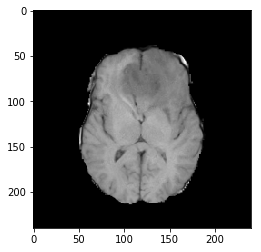
\includegraphics[width=14cm]{chapters/06_hdm/c_Brats18_2013_17_1_L1/41.png}
\caption{T1 modality scan}
\end{figure}

\subsection{T2}
The T2 modality measures


Gadolinium is a chemical compound given during MRI scans that highlights areas of inflammation.


\begin{itemize}
    \item Native (T1)
    \item Post-contrast T1-weighted (T1Gd)
    \item T2-weighted (T2)
    \item T2 Fluid Attenuated Inversion Recovery (FLAIR)
\end{itemize}